\SetKw{State}{state}
\SetKw{Send}{send}
\SetKw{Wait}{wait}
\SetKw{Call}{call}
\SetKw{Return}{return}

\SetKwComment{Comment}{//}{}

\SetKwProg{Function}{function}{}{end}

\SetKwBlock{parallelblk}{Do In Parallel}{end}
\SetKwBlock{atomicblk}{atomic}{end}

\SetKwFunction{atomicAdd}{AtomicAdd}
\SetKwFunction{sortps}{sortByPredecessorSize}
\SetKwFunction{clientSubmit}{Client::SubmitOp}
\SetKwFunction{clientWait}{Client::WaitOp}
\SetKwFunction{leaderSubmit}{Leader::SubmitOpRecv}
\SetKwFunction{replicaCoord}{Replica::coordRequestRecv}
\SetKwFunction{shardMain}{Leader::shardMain}
\SetKwFunction{CR}{Leader::CoordinationRequest}
\SetKwFunction{CRReply}{Leader::CoordinationResponse}
\SetKwFunction{append}{.append}
\SetKwFunction{find}{.find}
\SetKwFunction{popO}{.popOrderedAndStale()}

\algnewcommand{\IfThenElse}[3]{% \IfThenElse{<if>}{<then>}{<else>}
  \algorithmicif\ #1\ \algorithmicthen\ #2\ \algorithmicelse\ #3}

\algnewcommand{\IfThen}[2]{% \IfThenElse{<if>}{<then>}{<else>}
  \algorithmicif\ #1\ \algorithmicthen\ #2}

\section{MDL Protocol}
\label{sec:design}
% 1. what are the key features it needs to do. which component of the protocol does that.
% 2. include parts in the motivation that describe why you can't simply do "X". and then in design you can refer to motivation...

\mdl is an extension of \sdl that, in addition to defining behavior for concurrency across clients, introduces the capability for concurrency per clients. Clients are front-end applications, running on webservers, that submit requests to stateful services, such as databases or kv-stores, running on storage servers located within the same datacenter or different datacenters as the webservers.

Existing protocols that provide \sdl assume clients abide by the restriction to single-dispatch requests, having at most one outstanding request at a time. This assumption comes from the definition of linearizability, which requires individual clients to behave sequentially. These protocols, such as Paxos, Raft, Viewstamped Replication, Zab, do not provide any guarantees on the order that concurrent requests issued from a single client take effect. Our definition of \md specifies that concurrent requests issued from a single client take effect in invocation order. 

\begin{figure}[!htb]
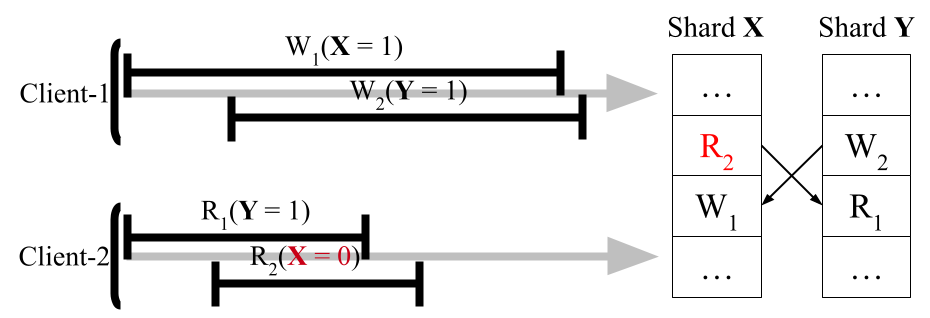
\includegraphics[scale=.45]{somet.png}
\caption{Example execution where two concurrent clients each submit 2 concurrent requests. Assume keys \textbf{X} and \textbf{Y} are at different shards. It is possible that $R_2$ arrives before $W_1$ at shard \textbf{X}, and $W_2$ arrives before $R_1$ at shard \textbf{Y}. Since clients expect their concurrent requests to take affect in invocation order, if $R_1$ returns 1, then $W_1$ must have taken affect before $R_1$, so $R_2$ should necessarily return a value of 1.}
\label{fig:concurrentbatches}
\end{figure}

\begin{figure}[!htb]
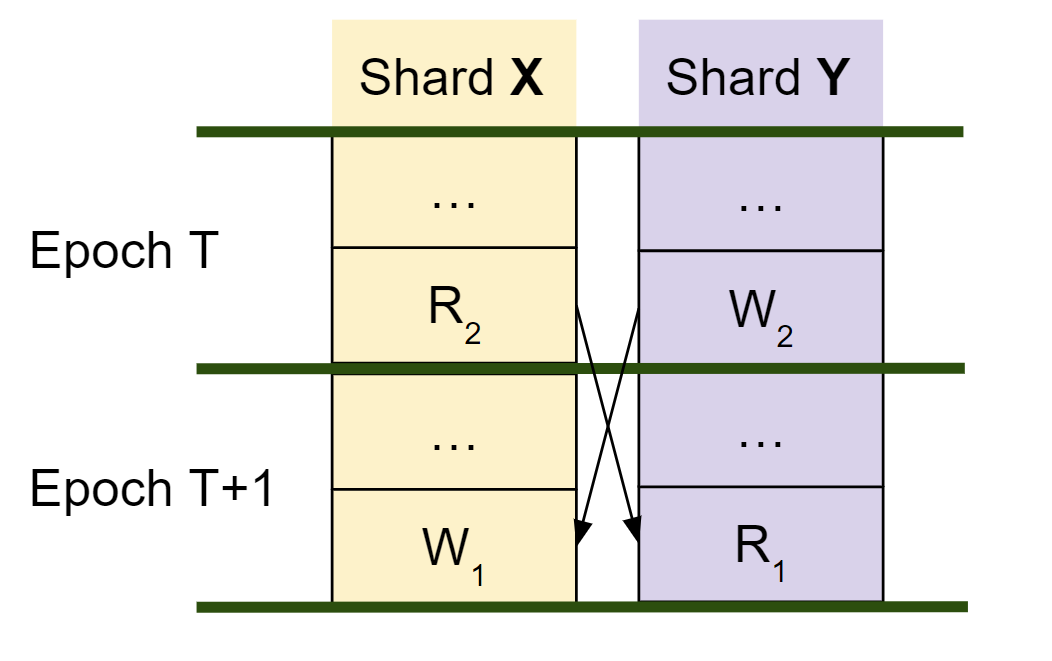
\includegraphics[scale=.3]{sorted_batching_wrong.png}
\caption{Example execution of sorted batching without coordination requirement. This execution leads to an incorrect execution that contains a cycle and is not \mdl. The execution is the same execution as that of figure \ref{fig:concurrentbatches}, but now the second request issued by each client arrives in an earlier epoch. Even if sorted in their respective epochs, they are not ordered across epochs without coordination.}
\label{fig:sortedbatchingwrong}
\end{figure}

For the single-shard setting, existing protocols come close to providing \mdl. A simple mechanism, such as per-client sequence numbers, can provide enough information for a shard leader to support invocation order for multiple requests from a single client. Such a solution does not suffice in the multi-shard setting, however, as shown in figure ~\ref{fig:concurrentbatches}. \sdl is a local property, thus a single-shard protocol correctly scales to multiple shards.  \mdl, however, is not a local property due to the possible interleaving of sets of concurrent requests across concurrent clients. This requires an \md protocol to use inter-shard communication in order to guarantee a safe total ordering that reflects issue order.

To support \mdl, we introduce a new protocol design, \md. This new design ensures the existing guarantees of \sdl such as (1) a total order of all requests that (2) respects real time ordering, as well as a new guaranty that (3) the total order respects per-client invocation-order. In this section we describe our protocol and how each component works to provide these guarantees.

\subsection{Overview}
The full client and shard protocols are specified in Algorithms ~\ref{clientprotocol} and ~\ref{shardprotocol}, respectively. Our protocol builds atop Raft, which provides \sdl. 

The key insight our protocol is designed around is the observation that if all requests in an execution are sorted in ascending order by the number of outstanding predecessors, or predecessor set size, then a safe total order will always exist. This derives from the guarantee that every cycle in an \md execution would need to contain at least two requests at the same shard where the first one executed has a larger predecessor set size than the second. More details are provided in our complete proof ~\ref{}. 

Since all requests can not be known a priori, we make use of epochs at each shard, and guarantee sorted execution order within each epoch, as well as a safe ordering across epochs. With this approach, we can prune request interleavings that might lead to cycles upfront, rather than running cycle detection and subsequently failing execution. While this unnecessarily prevents some subset of safe interleavings, the latter scales poorly for very large cycles.

\subsection{Per Client Invocation Order}

We use per-client sequence numbers to enforce invocation order at each individual shard. Sequence numbers are assigned at the client library 
and increase monotonically per shard. For example, a client issuing two requests for the first time to different keys that are on different shards will issue two requests both with sequence number 0. The shard leaders can then easily detect when a client's request
has arrived out of order and can buffer it until the necessary predecessor requests intended for the same shard arrive.

To support invocation order across shards, we introduce a message type for inter-shard communication, called a coordination request (CR). 
When each client submits a request to a shard, in parallel it also submits a coordination request to 
the shard of its predecessor. For some request issued by client C that has sequence number $s$, a predecessor request is defined as 
the concurrent request that client C issued with sequence number $s-1$. If client C does not
have any other outstanding requests, then the predecessor is nil.

Requests can only be executed in a given epoch if they have also been coordinated by their predecessor, which is signaled when the shard
leader of the predecessor responds success for the CR message. Requests with 0 predecessors are vacuously coordinated. Importantly, a shard can only coordinate
a request if the predecessor itself is also coordinated (and committed). This inductively guarantees that all concurrent requests that were previously invoked
will be coordinated, and thus sorted in their epochs. This is also why clients only need to submit a single CR to the single outstanding predecessor.

% To to get invocation order, there are multiple mechanisms at play
% 1. sequence numbers
% 2. CR requests that are issued by clients
%       -these only get sent to the immediate predecessor (talk about inductive guarantees)
%       -these only get acked if all the other predecessors have been acked too, guaranteeing they are sorted as well. you can only be in an epoch equivalent to or greater than the epochs of your predecessors (not absolute values)

\subsection{Total Order}
A total execution order is guaranteed by ensuring shards sort \textit{ordered} requests by increasing size of predecessor set within each epoch and execute requests in monotonically increasing epoch order. As mentioned before, sorting requests by the number of predecessors ensures a safe total ordering exists. The client library keeps track of the total number of outstanding requests at a given time, which it submits with each request for its predecessor set size. Requests with equal predecessor set sizes are sorted by arrival order to guarantee a stable sort across replicas.

An \textit{ordered} request is one that has been committed and coordinated. \md commits requests with the same mechanism as regular Raft, and it coordinates requests with the use of CR messages sent between shard leaders. Since executing requests now depends on two requirements being fulfilled, commitment as well as coordination, shards keep track of two logs. The first is an execution log containing \textit{ordered} requests that is segmented by epochs, and the second is a buffered log where request entries exist until they are committed (replicated at a majority) and coordinated. While this could be achieved with one log that contains holes and is executed in custom nonlinear order, we choose to break the log into two logs to simplify things and to remain consistent with Raft. We include a final \textit{ordering} inter-replica agreement at the end of each epoch to move requests between logs.

\md can only guarantee a safe total ordering across epochs of shards if it executes \textit{ordered} requests. Figure ~\ref{fig:sortedbatchingwrong} shows an execution that does not abide by this constraint, and only sorts committed (but not coordinated) requests within epochs. A cycle arises among all the requests across epoch boundaries, thus the execution does not have a total order and is not multi-dispatch linearizeable. A SUCCESS response for a given request's CR message, which coordinates it, serves as a promise that all predecessors have been sorted at the same or earlier epochs on their respective shards, which provides a total order across epochs of different shards.

\subsubsection{Failure Semantics}
We define \mdl failures as follows: a group of outstanding requests issued by a client will induce a prefix-closed set of success responses followed by a set of failed responses. It is possible that all of the requests succeed, and the set of failed responses will be empty. Importantly, if a request fails, all concurrent requests invoked by the same client with greater sequence numbers will also fail.

The coordination mechanism that we use to ensure correct ordering across epochs also satisfies these specific failure properties. A request can fail in one of two ways: (1) it times out while waiting to be coordinated, which we implement by bounding the number of epochs during which it can exist in the buffered log, or (2) it receives an explicit FAIL response for its CR message. With the inductive guarantees from CR messages, once a request fails it is guaranteed all subsequent requests will also fail.
% Ensure that epcoh increase monotonically
% ensure that each epoch is executed in sorted order
% ensure that across epoch boundaries nothing fishy happens, guaranteed via CR acks
% ensure we have the extra round trip at the end to "order" commands (this is for failure too??)

\subsection{Batching}
\md makes use of batching to increase throughput and amortize the \textit{ordering} inter-replica round trip across multiple requests in an epoch. Multi-dispatch linearizeable back-end systems expect to experience more load than their single-dispatch linearizeable counterparts, since individual clients can issue many more requests in the former. For example, for $k$ shards, if clients submit on average 10 requests at a time, the logs at shards of \md backends will be about $10/k$ times longer than the logs of \sd shards. Thus batching is a nice way to handle processing of congested shard logs. Moreover, our coordination mechanism is independent across requests from different clients, thus we do not introduce any head-of-line blocking. For requests that arrive later but become coordinated sooner, those can be executed immediately without waiting on the coordination of requests from separate clients.
% Comment that we expect a more congested log at each shard since now there will be fanout from individual clients
% batching is a nice fit since it can exploit this high load
% moreover, ordering a request does not depend on previously arrived requests from independent clients to be ordered, hwich is a nice design that allows each client to see issue order scale with just their behavior, not other clients'.

\subsection{Correctness}
We provide a full proof of correctness in ~\ref{}.

\subsection{Leader Failure}
% what are our failure semantics?


%%%%%%%%%%%%%%%%%%%%%%%%%%%%%%%%%
%%%%%%%%% Client %%%%%%%%%%%%%%%%
%%%%%%%%%%%%%%%%%%%%%%%%%%%%%%%%%
\begin{algorithm}
    \State $PID \gets$ unique client ID\\
    \State $\mathcal{L} \gets \{...\}$ \algorithmiccomment{Shard Leaders}\\
    \State $i \gets 0$ \algorithmiccomment{Sequence No Per Shard}\\
    \State $prevReq \gets NULL$\\
    \State $P \gets 0$
    \State $m$ \algorithmiccomment{mutex}\\
    \Function{\clientSubmit{Op, K, V}}{\\
        $seqno := \atomicAdd(i, 1)$\\
        $Req := (Op, K, V, PID, seqno)$\\
        $m.lock()$ \algorithmiccomment{Critical section begins}\\
        $prq := prevReq$\\
        $prevReq \gets Req$\\
        $P++$\\
        $m.unlock()$ \algorithmiccomment{Critical section begins}\\
        \IfThen{$prevReq \neq NULL$}{\Send $SubmitCR(prq, Req, P)$ to $L_{K-1} \in \mathcal{L}$}\\
        \Send $SubmitOp(Req)$ to $L_K \in \mathcal{L}$\\        
    }

    \Function{\clientWait{Req}}{
        \Wait receive $SubmitOpReply(V)$ from $L_K \in \mathcal{L}$\\
        $m.lock()$\\
        $\IfThen{prevReq = Req}{prevReq \gets NULL}$\\
        $m.unlock()$\\
        \Return $V$\\
    }
    \caption{MD-Lin Client}
    \label{clientprotocol}
\end{algorithm}
%%%%%%%%%%%%%%%%%%%%%%%%%%%%%%%%%
%%%%% Shard Leader %%%%%%%%%%%%%%
%%%%%%%%%%%%%%%%%%%%%%%%%%%%%%%%%
\begin{algorithm}
    \State $Epoch \gets 0$\\
    \State $Timer \gets T$\\
    \State $accepting \getst True$\\
    \State $commitLog \gets []$\\
    \State $orderedLog \gets []$\\
    \State $ClientSeqnoMap \gets [][]$\\
    \Function{\shardMain{}}{
        \Wait until $Timer = 0$\\
        $accepting \gets False$\\
        $batch := []$\\
        \For{$entry \in commitLog$}{\\
            \If{$entry.committed \land entry.coordinated$}{\\
                $entry.epoch \gets Epoch$\\
                $batch\append{entry}$\\
            }
        }
        \sortps{batch}\\
        $orderedLog\append{batch}$\\
        \Send $AppendEntries(batch, Epoch)$ to all $r \in \mathcal{R}$\\
        \Wait receive $AppendEntriesSuccess$ from all $r \in Q \in \mathcal{R}$\\
        $commitLog\popO{}$\\
        $\atomicAdd(Epoch, 1)$\\
        $accepting \gets True$\\
        $Timer \gets T$
        
    }
    \Function{\leaderSubmit{Op, K, V, P, s}}{
        \If{$ClientSeqnoMap[P] \neq s$}{
            $buffer_{P}(\{Op, K, V, P, s, bd\})$\\
            \Return\\
        }
        \Wait until $accepting = True$\\
        \For{$entry \in buffer_{P}$}{
            $commitLog\append{entry}$\\
            $ClientSeqnoMap[P]++$\\
            \Send $AppendEntries(entry)$ to all $r \in \mathcal{R}$\\
        }
        \Wait receive $AppendEntriesSuccess$ from all $r \in Q \in \mathcal{R}$ for all $entry \in buffer_{P}$\\
        $entry.committed \gets True$ for all $entry \in buffer_{P}$ that received $Success$\\
    }
    \Function{\CR{prq, rq}}{
        \If{$orderedLog\find{prq} \neq NULL$}{
            \Return asdkfsdf\\
        }
    }
    \Function{\CRReply{rq, v}}{
    
    }
    \caption{MD-Lin Shard Leader}
    \label{shardprotocol}
\end{algorithm}